\section{Hardness result on a line}
\label{npline}


%In 2022 Erlebach et al.~\cite{erlebach:drones} showed that the Drone Delivery Problem is NP-hard for general graphs, as well as the special case on the line\cite{erlebach:drones}. 
%Their construction in the case of the delivery on a line it is necessary that there are different speeds in order of input size.  We take another step and show that the problem remains NP-hard even if we restrict the instance to agents of only two different speeds. For that, we show a reduction from Partition to the aforementioned problem. The Partition problem is a very well studied NP-complete problem providing a convenient structure for our proof \cite{garey1979computers}. Our reduction closes the gap between trivially solvable instances with one speed (all agents move towards and follow the package) and previously known results with $O(n)$ speeds. We will refer to delivery on a line as DDTL.

For the problem on a line, it is intuitive to conceptualize the drones' movement areas as a series of intervals. Specifically, for an agent $a$ with its movement area $V_a$ connected by edges $E_a$, we can represent $a$ as an interval $[u,u']$, where $u$ is the leftmost vertex of $V_a$  and $u'$ is the rightmost vertex. This interval notation helps simplify the representation of each agent’s range of movement on the line, facilitating easier analysis of their interactions and potential overlap within the path graph.  Figure~\ref{fig:DDTlineexample} gives an example.
%\todo{S: kelin could you also add a dot at $p_4$?}
    \begin{figure}
        \centering
        \includegraphics[scale=0.55]{figures/DDTlineexamplenew.png}
        \caption{An example of a DDT-Line instance and its optimal solution is depicted: The solid line from $s$ to $y$ forms the path graph, where each solid edge has a distance of $1$. The initial positions of four drones are $p_1=s, p_2, p_3, p_4$, with the solid lines above and below representing each drone's movement subgraph. Suppose drone $1$ and $2$ have a speed of $1$, drone $3$ and drone $4$ have a speed of $3$. The optimal solution for this example takes a total time of $ \max\{1, 3/3\} + 3/3 + 3 = 5$ by sequentially using drones $1 $,  $ 3$ and $ 2$ to deliver the package from  $s$ to $y$, as indicated by the bold solid arrows. The dashed arrows represent the respective empty phases.} 
        \label{fig:DDTlineexample}
    \end{figure}
 

The hardness of the DDT problem on a line (DDT-Line) was first demonstrated in~\cite{erlebach:drones}. Their construction requires that all drones have varying speeds proportional to the input size.  Furthermore, they noted that the DDT-Line can be solved in polynomial time if all drones operate at the same speed, as all agents would simply move towards and follow the package. 
We advance this research by showing that the problem remains NP-hard even if we limit the scenario to agents with only two different speeds. 

\thmline*

We achieve this through a reduction from the well-studied NP-complete Partition problem~\cite{garey1979computers}, which provides a convenient structure for our proof. This reduction closes the gap between trivially solvable instances with unit speed, and the more complex scenarios previously established with $O(k)$ different speeds. First we discuss the construction and high level idea of the construction and later in the section we state a formal proof.

Let a set of positive integers $M= \{p_1,...,p_n\}$ be a partition problem instance with $ |M|= n$ and $P=\sum_{i\in [n]} p_i$. Without loss of generality, we assume that the numbers in $M$ are arranged in non-descending order, i.e.\ $p_i\leq p_j, \forall i<j$. The Partition problem involves determining whether there exists a partition $S\subset M$ such that $\sum_{S}p_i=\sum_{M\setminus S}p_i$.  In our DDT-Line instance, 
 we want each $p_i$ to be associated with an agent in DDT-Line and to offer two options: help on the left-side path or help on the right-side path. Then, we construct the scenario where the optimal (fastest) schedule is achieved if and only if the agents are arranged so that the sum of their associated integers 
on both sides equals exactly $\frac{P}{2}$. 

We now begin constructing an instance for the DDT-Line.    
To assist with the illustration, we have provided two figures:  
Figure \ref{fig:line_2speed} shows the layout of all drones' operating areas within a path graph, while Figure \ref{fig:line_2speed_gadget} provides a detailed view of the construction. Two different speeds are represented by colors in both Figure~s: red for the fast agents and black for the slow ones.    
%\textcolor{blue}{Without loss of generality, We assume the numbers in $M$ are arranged in ascending order., i.e.\ $p_i\leq p_j, \forall i<j$. Then, }

For every $p_i$ from the Partition instance, we associate one slow agent $e_i$ (referred to as the \emph{element agent}), two fast agents $f_i^{l}$ and $f_i^{r}$, as well as two slow agents $b_i^l$ and $b_i^r$ (referred to as the \emph{base agents}) for the DDT-Line.  
For every $b_i^l$ (resp, $b_i^r$), there is a fast agent $h_i^l$ (resp, $h_i^r$) (referred to as the \emph{helping agents}).  For simplification, we use $b_i$ (resp. $ h_i $, $ f_i$) to denote either $b^l_i$ and  $b^r_i$ (resp, $h^l_i$ and  $h^r_i$, $f^l_i$ and  $f^r_i$). 
Additionally we have the slow auxiliary agents $d$ and $p$, as well as the fast auxiliary agent $q$. Agent $d$ serves as a \emph{delay}. Every feasible schedule has to assign the package to $d$ to initiate delivery from starting point $s$ and wait for it to traverse the interval of $d$. By selecting an appropriate length for $d$, we ensure that there is sufficient time for the $e_i$ agents to reach their designated helping spot (empty phase). Note that this \emph{delay} is a commonly employed technique in constructing hardness proofs for the DDT.   

\begin{figure}[ht]
    \centering
    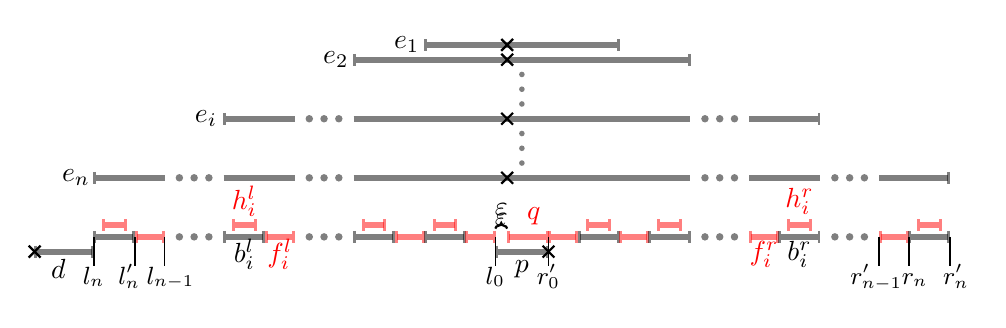
\begin{tikzpicture}[scale=0.75]
\definecolor{dgreen}{RGB}{0, 0, 0}
\usetikzlibrary{decorations.pathreplacing}
\draw[dgreen, opacity=0.5, line width=2.25pt]   (0.037500000000000006, 0) -- (0.9625, 0);
\draw[dgreen, opacity=0.5, line width=0.037500000000000006*1cm/1pt]      (0.018750000000000003, 0.1) -- (0.018750000000000003, -0.1);
\draw[dgreen, opacity=0.5, line width=0.037500000000000006*1cm/1pt]      (0.98125, 0.1) -- (0.98125, -0.1);
\node at (0.7, 1.25)  { $e_n$};
\draw[black, opacity=0.5, line width=2.25pt]   (1.0375, 1.25) -- (2.2, 1.25);
\draw[black, opacity=0.5, line width=0.037500000000000006*1cm/1pt]      (1.01875, 1.35) -- (1.01875, 1.15);
\node at (2.9000000000000004, 1.25)  { };
\draw[black, opacity=0.5, line width=2.25pt]   (3.2, 1.25) -- (4.4, 1.25);
\node at (2.9000000000000004, 2.25)  { $e_i$};
\draw[black, opacity=0.5, line width=2.25pt]   (3.2375000000000003, 2.25) -- (4.4, 2.25);
\draw[black, opacity=0.5, line width=0.037500000000000006*1cm/1pt]      (3.21875, 2.35) -- (3.21875, 2.15);
\node at (5.1000000000000005, 1.25)  { };
\draw[black, opacity=0.5, line width=2.25pt]   (5.4, 1.25) -- (11.099999999999998, 1.25);
\node at (5.1000000000000005, 2.25)  { };
\draw[black, opacity=0.5, line width=2.25pt]   (5.4, 2.25) -- (11.099999999999998, 2.25);
\node at (5.1000000000000005, 3.25)  { $e_2$};
\draw[black, opacity=0.5, line width=2.25pt]   (5.4375, 3.25) -- (11.062499999999998, 3.25);
\draw[black, opacity=0.5, line width=0.037500000000000006*1cm/1pt]      (5.41875, 3.35) -- (5.41875, 3.15);
\draw[black, opacity=0.5, line width=0.037500000000000006*1cm/1pt]      (11.081249999999997, 3.35) -- (11.081249999999997, 3.15);
\node at (6.300000000000001, 3.5)  { $e_1$};
\draw[black, opacity=0.5, line width=2.25pt]   (6.6375, 3.5) -- (9.862499999999999, 3.5);
\draw[black, opacity=0.5, line width=0.037500000000000006*1cm/1pt]      (6.61875, 3.6) -- (6.61875, 3.4);
\draw[black, opacity=0.5, line width=0.037500000000000006*1cm/1pt]      (9.881249999999998, 3.6) -- (9.881249999999998, 3.4);
\node at (11.799999999999997, 1.25)  { };
\draw[black, opacity=0.5, line width=2.25pt]   (12.099999999999998, 1.25) -- (13.299999999999997, 1.25);
\node at (11.799999999999997, 2.25)  { };
\draw[black, opacity=0.5, line width=2.25pt]   (12.099999999999998, 2.25) -- (13.262499999999998, 2.25);
\draw[black, opacity=0.5, line width=0.037500000000000006*1cm/1pt]      (13.281249999999996, 2.35) -- (13.281249999999996, 2.15);
\node at (13.999999999999996, 1.25)  { };
\draw[black, opacity=0.5, line width=2.25pt]   (14.299999999999997, 1.25) -- (15.462499999999997, 1.25);
\draw[black, opacity=0.5, line width=0.037500000000000006*1cm/1pt]      (15.481249999999996, 1.35) -- (15.481249999999996, 1.15);
\draw[dgreen, opacity=0.5, line width=2.25pt]   (1.0375, 0.25) -- (1.6624999999999999, 0.25);
\draw[dgreen, opacity=0.5, line width=0.037500000000000006*1cm/1pt]      (1.01875, 0.35) -- (1.01875, 0.15);
\draw[dgreen, opacity=0.5, line width=0.037500000000000006*1cm/1pt]      (1.68125, 0.35) -- (1.68125, 0.15);
\draw[red, opacity=0.5, line width=2.25pt]   (1.1875, 0.45) -- (1.5125, 0.45);
\draw[red, opacity=0.5, line width=0.037500000000000006*1cm/1pt]      (1.16875, 0.55) -- (1.16875, 0.35);
\draw[red, opacity=0.5, line width=0.037500000000000006*1cm/1pt]      (1.53125, 0.55) -- (1.53125, 0.35);
\draw[red, opacity=0.5, line width=2.25pt]   (1.7375, 0.25) -- (2.1625, 0.25);
\draw[red, opacity=0.5, line width=0.037500000000000006*1cm/1pt]      (1.71875, 0.35) -- (1.71875, 0.15);
\draw[red, opacity=0.5, line width=0.037500000000000006*1cm/1pt]      (2.1812500000000004, 0.35) -- (2.1812500000000004, 0.15);
\draw[dgreen, opacity=0.5, line width=2.25pt]   (3.2375000000000003, 0.25) -- (3.8625000000000003, 0.25);
\draw[dgreen, opacity=0.5, line width=0.037500000000000006*1cm/1pt]      (3.21875, 0.35) -- (3.21875, 0.15);
\draw[dgreen, opacity=0.5, line width=0.037500000000000006*1cm/1pt]      (3.8812500000000005, 0.35) -- (3.8812500000000005, 0.15);
\draw[red, opacity=0.5, line width=2.25pt]   (3.3875, 0.45) -- (3.7125000000000004, 0.45);
\draw[red, opacity=0.5, line width=0.037500000000000006*1cm/1pt]      (3.36875, 0.55) -- (3.36875, 0.35);
\draw[red, opacity=0.5, line width=0.037500000000000006*1cm/1pt]      (3.7312500000000006, 0.55) -- (3.7312500000000006, 0.35);
\draw[red, opacity=0.5, line width=2.25pt]   (3.9375000000000004, 0.25) -- (4.362500000000001, 0.25);
\draw[red, opacity=0.5, line width=0.037500000000000006*1cm/1pt]      (3.91875, 0.35) -- (3.91875, 0.15);
\draw[red, opacity=0.5, line width=0.037500000000000006*1cm/1pt]      (4.3812500000000005, 0.35) -- (4.3812500000000005, 0.15);
\draw[dgreen, opacity=0.5, line width=2.25pt]   (5.4375, 0.25) -- (6.062500000000001, 0.25);
\draw[dgreen, opacity=0.5, line width=0.037500000000000006*1cm/1pt]      (5.41875, 0.35) -- (5.41875, 0.15);
\draw[dgreen, opacity=0.5, line width=0.037500000000000006*1cm/1pt]      (6.081250000000001, 0.35) -- (6.081250000000001, 0.15);
\draw[red, opacity=0.5, line width=2.25pt]   (5.5875, 0.45) -- (5.9125000000000005, 0.45);
\draw[red, opacity=0.5, line width=0.037500000000000006*1cm/1pt]      (5.5687500000000005, 0.55) -- (5.5687500000000005, 0.35);
\draw[red, opacity=0.5, line width=0.037500000000000006*1cm/1pt]      (5.93125, 0.55) -- (5.93125, 0.35);
\draw[red, opacity=0.5, line width=2.25pt]   (6.1375, 0.25) -- (6.562500000000001, 0.25);
\draw[red, opacity=0.5, line width=0.037500000000000006*1cm/1pt]      (6.11875, 0.35) -- (6.11875, 0.15);
\draw[red, opacity=0.5, line width=0.037500000000000006*1cm/1pt]      (6.581250000000001, 0.35) -- (6.581250000000001, 0.15);
\draw[dgreen, opacity=0.5, line width=2.25pt]   (6.6375, 0.25) -- (7.262500000000001, 0.25);
\draw[dgreen, opacity=0.5, line width=0.037500000000000006*1cm/1pt]      (6.61875, 0.35) -- (6.61875, 0.15);
\draw[dgreen, opacity=0.5, line width=0.037500000000000006*1cm/1pt]      (7.281250000000001, 0.35) -- (7.281250000000001, 0.15);
\draw[red, opacity=0.5, line width=2.25pt]   (6.7875000000000005, 0.45) -- (7.112500000000001, 0.45);
\draw[red, opacity=0.5, line width=0.037500000000000006*1cm/1pt]      (6.768750000000001, 0.55) -- (6.768750000000001, 0.35);
\draw[red, opacity=0.5, line width=0.037500000000000006*1cm/1pt]      (7.1312500000000005, 0.55) -- (7.1312500000000005, 0.35);
\draw[red, opacity=0.5, line width=2.25pt]   (7.3375, 0.25) -- (7.762500000000001, 0.25);
\draw[red, opacity=0.5, line width=0.037500000000000006*1cm/1pt]      (7.3187500000000005, 0.35) -- (7.3187500000000005, 0.15);
\draw[red, opacity=0.5, line width=0.037500000000000006*1cm/1pt]      (7.781250000000001, 0.35) -- (7.781250000000001, 0.15);
\draw[dgreen, opacity=0.5, line width=2.25pt]   (7.8375, 0) -- (8.6625, 0);
\draw[dgreen, opacity=0.5, line width=0.037500000000000006*1cm/1pt]      (7.8187500000000005, 0.1) -- (7.8187500000000005, -0.1);
\draw[dgreen, opacity=0.5, line width=0.037500000000000006*1cm/1pt]      (8.681249999999999, 0.1) -- (8.681249999999999, -0.1);
\draw[red, opacity=0.5, line width=2.25pt]   (8.0375, 0.25) -- (8.6625, 0.25);
\draw[red, opacity=0.5, line width=0.037500000000000006*1cm/1pt]      (8.01875, 0.35) -- (8.01875, 0.15);
\draw[red, opacity=0.5, line width=0.037500000000000006*1cm/1pt]      (8.681249999999999, 0.35) -- (8.681249999999999, 0.15);
\draw[red, opacity=0.5, line width=2.25pt]   (8.737499999999999, 0.25) -- (9.1625, 0.25);
\draw[red, opacity=0.5, line width=0.037500000000000006*1cm/1pt]      (8.71875, 0.35) -- (8.71875, 0.15);
\draw[red, opacity=0.5, line width=0.037500000000000006*1cm/1pt]      (9.181249999999999, 0.35) -- (9.181249999999999, 0.15);
\draw[dgreen, opacity=0.5, line width=2.25pt]   (9.237499999999999, 0.25) -- (9.862499999999999, 0.25);
\draw[dgreen, opacity=0.5, line width=0.037500000000000006*1cm/1pt]      (9.21875, 0.35) -- (9.21875, 0.15);
\draw[dgreen, opacity=0.5, line width=0.037500000000000006*1cm/1pt]      (9.881249999999998, 0.35) -- (9.881249999999998, 0.15);
\draw[red, opacity=0.5, line width=2.25pt]   (9.3875, 0.45) -- (9.712499999999999, 0.45);
\draw[red, opacity=0.5, line width=0.037500000000000006*1cm/1pt]      (9.36875, 0.55) -- (9.36875, 0.35);
\draw[red, opacity=0.5, line width=0.037500000000000006*1cm/1pt]      (9.731249999999998, 0.55) -- (9.731249999999998, 0.35);
\draw[red, opacity=0.5, line width=2.25pt]   (9.937499999999998, 0.25) -- (10.362499999999999, 0.25);
\draw[red, opacity=0.5, line width=0.037500000000000006*1cm/1pt]      (9.91875, 0.35) -- (9.91875, 0.15);
\draw[red, opacity=0.5, line width=0.037500000000000006*1cm/1pt]      (10.381249999999998, 0.35) -- (10.381249999999998, 0.15);
\draw[dgreen, opacity=0.5, line width=2.25pt]   (10.437499999999998, 0.25) -- (11.062499999999998, 0.25);
\draw[dgreen, opacity=0.5, line width=0.037500000000000006*1cm/1pt]      (10.41875, 0.35) -- (10.41875, 0.15);
\draw[dgreen, opacity=0.5, line width=0.037500000000000006*1cm/1pt]      (11.081249999999997, 0.35) -- (11.081249999999997, 0.15);
\draw[red, opacity=0.5, line width=2.25pt]   (10.587499999999999, 0.45) -- (10.912499999999998, 0.45);
\draw[red, opacity=0.5, line width=0.037500000000000006*1cm/1pt]      (10.56875, 0.55) -- (10.56875, 0.35);
\draw[red, opacity=0.5, line width=0.037500000000000006*1cm/1pt]      (10.931249999999997, 0.55) -- (10.931249999999997, 0.35);
\draw[red, opacity=0.5, line width=2.25pt]   (12.137499999999998, 0.25) -- (12.562499999999998, 0.25);
\draw[red, opacity=0.5, line width=0.037500000000000006*1cm/1pt]      (12.118749999999999, 0.35) -- (12.118749999999999, 0.15);
\draw[red, opacity=0.5, line width=0.037500000000000006*1cm/1pt]      (12.581249999999997, 0.35) -- (12.581249999999997, 0.15);
\draw[dgreen, opacity=0.5, line width=2.25pt]   (12.637499999999998, 0.25) -- (13.262499999999998, 0.25);
\draw[dgreen, opacity=0.5, line width=0.037500000000000006*1cm/1pt]      (12.618749999999999, 0.35) -- (12.618749999999999, 0.15);
\draw[dgreen, opacity=0.5, line width=0.037500000000000006*1cm/1pt]      (13.281249999999996, 0.35) -- (13.281249999999996, 0.15);
\draw[red, opacity=0.5, line width=2.25pt]   (12.787499999999998, 0.45) -- (13.112499999999997, 0.45);
\draw[red, opacity=0.5, line width=0.037500000000000006*1cm/1pt]      (12.768749999999999, 0.55) -- (12.768749999999999, 0.35);
\draw[red, opacity=0.5, line width=0.037500000000000006*1cm/1pt]      (13.131249999999996, 0.55) -- (13.131249999999996, 0.35);
\draw[red, opacity=0.5, line width=2.25pt]   (14.337499999999997, 0.25) -- (14.762499999999998, 0.25);
\draw[red, opacity=0.5, line width=0.037500000000000006*1cm/1pt]      (14.318749999999998, 0.35) -- (14.318749999999998, 0.15);
\draw[red, opacity=0.5, line width=0.037500000000000006*1cm/1pt]      (14.781249999999996, 0.35) -- (14.781249999999996, 0.15);
\draw[dgreen, opacity=0.5, line width=2.25pt]   (14.837499999999997, 0.25) -- (15.462499999999997, 0.25);
\draw[dgreen, opacity=0.5, line width=0.037500000000000006*1cm/1pt]      (14.818749999999998, 0.35) -- (14.818749999999998, 0.15);
\draw[dgreen, opacity=0.5, line width=0.037500000000000006*1cm/1pt]      (15.481249999999996, 0.35) -- (15.481249999999996, 0.15);
\draw[red, opacity=0.5, line width=2.25pt]   (14.987499999999997, 0.45) -- (15.312499999999996, 0.45);
\draw[red, opacity=0.5, line width=0.037500000000000006*1cm/1pt]      (14.968749999999998, 0.55) -- (14.968749999999998, 0.35);
\draw[red, opacity=0.5, line width=0.037500000000000006*1cm/1pt]      (15.331249999999995, 0.55) -- (15.331249999999995, 0.35);
\draw[thick, decorate, decoration={brace, amplitude=2pt}] (7.800000000000001, 0.39) -- (8.0, 0.39) node[midway,yshift=7pt] {$\varepsilon$};
\draw[thick] (-0.1, -0.1) -- (0.1, 0.1);
\draw[thick] (0.1, -0.1) -- (-0.1, 0.1);
\draw[thick] (7.9, 1.15) -- (8.1, 1.35);
\draw[thick] (8.1, 1.15) -- (7.9, 1.35);
\draw[thick] (7.9, 2.15) -- (8.1, 2.35);
\draw[thick] (8.1, 2.15) -- (7.9, 2.35);
\draw[thick] (7.9, 3.15) -- (8.1, 3.35);
\draw[thick] (8.1, 3.15) -- (7.9, 3.35);
\draw[thick] (7.9, 3.4) -- (8.1, 3.6);
\draw[thick] (8.1, 3.4) -- (7.9, 3.6);
\draw[thick] (8.6, -0.1) -- (8.799999999999999, 0.1);
\draw[thick] (8.799999999999999, -0.1) -- (8.6, 0.1);
\node[] at (3.5500000000000003, -0.04999999999999999) {\color{dgreen}$b_i^l$};
\node[] at (3.5500000000000003, 0.85) {\color{red}$h_i^l$};
\node[] at (4.15, -0.04999999999999999) {\color{red}$f_i^l$};
\node[] at (12.949999999999998, 0.85) {\color{red}$h_i^r$};
\node[] at (12.949999999999998, -0.04999999999999999) {\color{dgreen}$b_i^r$};
\node[] at (12.349999999999998, -0.04999999999999999) {\color{red}$f_i^r$};
\node[] at (0.4, -0.3) {\color{dgreen}$d$};
\node[] at (8.25, -0.3) {\color{dgreen}$p$};
\node[] at (8.45, 0.6) {\color{red}$q$};
\node[] at (7.9, 0.55) {\color{black}$\varepsilon$};
\draw[black, line width=0.02*1cm/1pt] (1, 0.25) -- (1, -0.25);
\node[anchor=base] at (1, -0.55) {\small\color{black}$l_n$};
\draw[black, line width=0.02*1cm/1pt] (1.7, 0.25) -- (1.7, -0.25);
\node[anchor=base] at (1.5999999999999999, -0.55) {\small\color{black}$l_n'$};
\draw[black, line width=0.02*1cm/1pt] (14.799999999999997, 0.25) -- (14.799999999999997, -0.25);
\node[anchor=base] at (14.899999999999997, -0.55) {\small\color{black}$r_n$};
\draw[black, line width=0.02*1cm/1pt] (15.499999999999996, 0.25) -- (15.499999999999996, -0.25);
\node[anchor=base] at (15.599999999999996, -0.55) {\small\color{black}$r_n'$};
\draw[black, line width=0.02*1cm/1pt] (7.800000000000001, 0.25) -- (7.800000000000001, -0.25);
\node[anchor=base] at (7.800000000000001, -0.55) {\small\color{black}$l_0$};
\draw[black, line width=0.02*1cm/1pt] (8.7, 0.25) -- (8.7, -0.25);
\node[anchor=base] at (8.7, -0.55) {\small\color{black}$r_0'$};
\draw[black, line width=0.02*1cm/1pt] (2.2, 0.25) -- (2.2, -0.25);
\node[anchor=base] at (2.3000000000000003, -0.55) {\small\color{black}$l_{n-1}$};
\draw[black, line width=0.02*1cm/1pt] (14.299999999999997, 0.25) -- (14.299999999999997, -0.25);
\node[anchor=base] at (14.249999999999996, -0.55) {\small\color{black}$r_{n-1}'$};
\fill[opacity=0.5] (2.45, 0.25) circle (1.8pt);
\fill[opacity=0.5] (2.7, 0.25) circle (1.8pt);
\fill[opacity=0.5] (2.95, 0.25) circle (1.8pt);
\fill[opacity=0.5] (2.45, 1.25) circle (1.8pt);
\fill[opacity=0.5] (2.7, 1.25) circle (1.8pt);
\fill[opacity=0.5] (2.95, 1.25) circle (1.8pt);
\fill[opacity=0.5] (4.65, 0.25) circle (1.8pt);
\fill[opacity=0.5] (4.9, 0.25) circle (1.8pt);
\fill[opacity=0.5] (5.15, 0.25) circle (1.8pt);
\fill[opacity=0.5] (4.65, 1.25) circle (1.8pt);
\fill[opacity=0.5] (4.9, 1.25) circle (1.8pt);
\fill[opacity=0.5] (5.15, 1.25) circle (1.8pt);
\fill[opacity=0.5] (4.65, 2.25) circle (1.8pt);
\fill[opacity=0.5] (4.9, 2.25) circle (1.8pt);
\fill[opacity=0.5] (5.15, 2.25) circle (1.8pt);
\fill[opacity=0.5] (11.349999999999998, 0.25) circle (1.8pt);
\fill[opacity=0.5] (11.599999999999998, 0.25) circle (1.8pt);
\fill[opacity=0.5] (11.849999999999998, 0.25) circle (1.8pt);
\fill[opacity=0.5] (11.349999999999998, 1.25) circle (1.8pt);
\fill[opacity=0.5] (11.599999999999998, 1.25) circle (1.8pt);
\fill[opacity=0.5] (11.849999999999998, 1.25) circle (1.8pt);
\fill[opacity=0.5] (11.349999999999998, 2.25) circle (1.8pt);
\fill[opacity=0.5] (11.599999999999998, 2.25) circle (1.8pt);
\fill[opacity=0.5] (11.849999999999998, 2.25) circle (1.8pt);
\fill[opacity=0.5] (13.549999999999997, 0.25) circle (1.8pt);
\fill[opacity=0.5] (13.799999999999997, 0.25) circle (1.8pt);
\fill[opacity=0.5] (14.049999999999997, 0.25) circle (1.8pt);
\fill[opacity=0.5] (13.549999999999997, 1.25) circle (1.8pt);
\fill[opacity=0.5] (13.799999999999997, 1.25) circle (1.8pt);
\fill[opacity=0.5] (14.049999999999997, 1.25) circle (1.8pt);
\fill[opacity=0.5] (8.25, 1.5) circle (1.3499999999999999pt);
\fill[opacity=0.5] (8.25, 1.75) circle (1.3499999999999999pt);
\fill[opacity=0.5] (8.25, 2.0) circle (1.3499999999999999pt);
\fill[opacity=0.5] (8.25, 2.5) circle (1.3499999999999999pt);
\fill[opacity=0.5] (8.25, 2.75) circle (1.3499999999999999pt);
\fill[opacity=0.5] (8.25, 3.0) circle (1.3499999999999999pt);
\end{tikzpicture}%[Finished in 42ms]
    \caption{A sketch of the DDT-Line instance construction. There are $3n+2$ slow agents $\{e_i, b^l_i, b^r_i\}_{i\in [n]} \cup \{d, p\}$, $4n+1$ fast agents $\{f^l_i,f^r_i, h^l_i, h^r_i\}_{i\in [n]} \cup \{q\}$. The starting point $s$ is the leftmost node of agent $d$'s interval, and the destination $y$ is the rightmost point of agent $e_n$'s interval. In the middle part we have a gap of size $\varepsilon$ which can only be traversed by the $e_i$'s or $p$. Assigning $e_i$'s to the left side such that the respective $p_i$'s sum up to exactly $\frac{P}{2}$, the package meets $p$ at $l_0$ without waiting time.}
\label{fig:line_2speed}
\end{figure} 


Observe that in the DDT-Line instance, we have alternating slow ($b_i$) and fast ($f_i$) base agents covering the main part of the $s-y$ interval. These agents cover the entire range except for a small gap of length  $\varepsilon$ in the middle, which is covered by the designated package carrier $p$ as well as the element agents. However, the instance is designed in a way such that we will have to choose $p$ here to achieve optimal delivery time. The $f_i$ agents are strategically designed so that no optimal schedule can bypass them. For the intervals corresponding to $b_i$, we have two options: either stick entirely with $b_i$ or use $h_i$ and a feasible $e_i$. The idea is that agent $h_i$ only benefits our schedule if we deliver the package to it and then pick it up from its right-most point by ``another agent''; otherwise, simply staying with $b_i $ yields the same solution. This introduces the role of $e_i$ as the ``another agent''. An agent $e_i$ acts as the counterpart to $b_i$ by either delivering to or picking up from $h_i$'s interval. Although any $e_j$ with $j>i$ could also play the respective counterpart or even stand in for $b_i$, this will not happen for any optimal solution, as we will discuss later. A detailed illustration of the $b_i$ and $h_i$ construction is provided in Figure  \ref{fig:line_2speed_gadget}.  

\begin{figure}[ht]
    \centering
    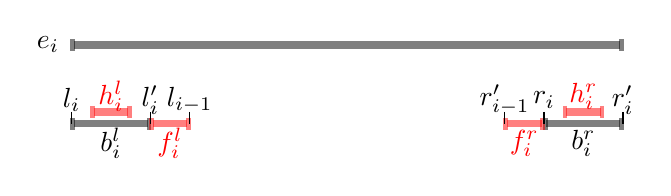
\begin{tikzpicture}[scale=0.5]
\definecolor{dgreen}{RGB}{13, 138, 8}
\draw[black, opacity=0.5, line width=2.7pt]   (11.06, 2) -- (24.94, 2);
\draw[black, opacity=0.5, line width=0.06*1cm/1pt]   (11.03, 2.15) -- (11.03, 1.85);
\draw[black, opacity=0.5, line width=0.06*1cm/1pt]   (24.97, 2.15) -- (24.97, 1.85);
\draw[black, opacity=0.5, line width=2.7pt]   (11.06, 0) -- (12.94, 0);
\draw[black, opacity=0.5, line width=0.06*1cm/1pt]   (11.03, 0.15) -- (11.03, -0.15);
\draw[black, opacity=0.5, line width=0.06*1cm/1pt]   (12.97, 0.15) -- (12.97, -0.15);
\draw[red, opacity=0.5, line width=2.7pt]   (11.56, 0.3) -- (12.44, 0.3);
\draw[red, opacity=0.5, line width=0.06*1cm/1pt]   (11.53, 0.44999999999999996) -- (11.53, 0.15);
\draw[red, opacity=0.5, line width=0.06*1cm/1pt]   (12.47, 0.44999999999999996) -- (12.47, 0.15);
\draw[red, opacity=0.5, line width=2.7pt]   (13.06, 0) -- (13.94, 0);
\draw[red, opacity=0.5, line width=0.06*1cm/1pt]   (13.03, 0.15) -- (13.03, -0.15);
\draw[red, opacity=0.5, line width=0.06*1cm/1pt]   (13.97, 0.15) -- (13.97, -0.15);
\draw[black, opacity=0.5, line width=2.7pt]   (23.06, 0) -- (24.94, 0);
\draw[black, opacity=0.5, line width=0.06*1cm/1pt]   (23.03, 0.15) -- (23.03, -0.15);
\draw[black, opacity=0.5, line width=0.06*1cm/1pt]   (24.97, 0.15) -- (24.97, -0.15);
\draw[red, opacity=0.5, line width=2.7pt]   (23.56, 0.3) -- (24.44, 0.3);
\draw[red, opacity=0.5, line width=0.06*1cm/1pt]   (23.53, 0.44999999999999996) -- (23.53, 0.15);
\draw[red, opacity=0.5, line width=0.06*1cm/1pt]   (24.47, 0.44999999999999996) -- (24.47, 0.15);
\draw[red, opacity=0.5, line width=2.7pt]   (22.06, 0) -- (22.94, 0);
\draw[red, opacity=0.5, line width=0.06*1cm/1pt]   (22.03, 0.15) -- (22.03, -0.15);
\draw[red, opacity=0.5, line width=0.06*1cm/1pt]   (22.97, 0.15) -- (22.97, -0.15);
\draw[black, line width=0.02*1cm/1pt]   (11, 0.3) -- (11, 0);
\draw[black, line width=0.02*1cm/1pt]   (13, 0.3) -- (13, 0);
\draw[black, line width=0.02*1cm/1pt]   (23, 0.3) -- (23, 0);
\draw[black, line width=0.02*1cm/1pt]   (25, 0.3) -- (25, 0);
\draw[black, line width=0.02*1cm/1pt]   (22, 0.3) -- (22, 0);
\draw[black, line width=0.02*1cm/1pt]   (14, 0.3) -- (14, 0);
\node[] at (12, -0.5) {\color{black}$b_i^l$};
\node[] at (13.5, -0.5) {\color{red}$f_i^l$};
\node[] at (24, -0.5) {\color{black}$b_i^r$};
\node[] at (22.5, -0.5) {\color{red}$f_i^r$};
\node[] at (10.4, 2) {\color{black}$e_i$};
\node[] at (12, 0.7) {\color{red}$h_i^l$};
\node[] at (24, 0.7) {\color{red}$h_i^r$};
\node[] at (14, 0.6) {\color{black}$l_{i-1}$};
\node[] at (11, 0.6) {\color{black}$l_i$};
\node[] at (13, 0.6) {\color{black}$l_i'$};
\node[] at (23, 0.6) {\color{black}$r_i$};
\node[] at (22, 0.6) {\color{black}$r_{i-1}'$};
\node[] at (25, 0.6) {\color{black}$r_i'$};
\end{tikzpicture}
    \caption{A close-up on $p_i$'s corresponding agents: slow agent $e_i$, $b_i^l $ and $ b_i^r$;  fast agents $f_i^l $, $ f_i^r$, $h_i^l$, and $ h_i^r$. From the construction, it is clear that  $e_i$ can only help only on either the left or right side interval, utilizing the fast drones $h_i$ on that side. A helping agent $h_i$ is utilized by assigning $e_i$ to either pick up the package from or deliver it to $h_i$. Not assigning $e_i$ leaves $h_i$ ineffective, as the delivery time is only dependent on $b_i$ as it has to catch up and pick up the package again.}
\label{fig:line_2speed_gadget}
\end{figure}


Building on the above observation, we will briefly outline the design goals for these intervals. 
It is important to note that the interval length of each agent $b_i$ depends on the underlying $p_i$, allowing us to construct both sides of the partition instance effectively. This means that the interval length of $b_i$ grows with the size $p_i$.  On the boundaries of the instance, the $b_i$'s have the largest lengths while they decrease as we move to the middle. It is clear that it benefits the delivery time the most if an element agent helps a larger $b_i$. To prevent any $e_i$ from helping any $b_j$ with $j>i$, we previously ordered the $p_i$ (and correspondingly the $e_i$) in increasing sequence and ensure that all $b_j$ with $j>i$ are inaccessible to $e_i$ (see Figure~\ref{fig:line_2speed}). As a result, $e_i$ can only help $b_j$ with $j\leq i$, while the optimal helping spot is then $b_i$ (either $b^l_i$ or  $b^r_i$). If $e_i$ would help at some $b_j$ with $j<i$ the schedule could be improved through an exchange argument. As large parts of the instance can be traversed with fast speed ($f_i$'s), it will not happen for any $e_i$ to help multiple $b_j$'s. This is exactly why there has to be made a choice between left and right by every $e_i$ to help a designated $b_j$ ($j\leq i$) which is $b_i^r$ or $b_i^l$ optimally.


To determine if the Partition instance is a ``yes''-instance, we use agent $p$. This agent is strategically positioned so that the package reaches agent $p$'s leftmost border precisely when the underlying $p_i$'s of the helping $e_i$'s sum up to exactly $\frac{P}{2}$ on the left side. Agent $p$ is positioned at its right border and upon initiating the delivery it starts moving to the left. Therefore we have to choose the length of $p$ to coincide with the exact time required to traverse the left side of the instance (including $d$) assuming we assign the $e_i$ agents corresponding to a feasible partition.
Only $p$ and all $e_i$ agents can traverse the middle part of our instance. The idea is that if we can not meet agent $p$ at the perfect time or use some agent $e_i$ instead of agent $p$ to traverse the middle gap, optimal delivery time cannot be achieved. %To make sure that $p$ does not help any $b_i^r$ (picking from or delivering the package to $h_i^r$), $p$ is (almost) completely covered by a fast agent $q$ which is supposed to travel over that middle part.   
Note that $p$ also cannot help any other $b_i^l$ or $b_i^r$ agents as there is no overlap between them.
There is another nuance to consider when it comes to the interval lengths of the agents $\{b^l_i\}_{i\in [n]}$. Assume for a moment that $b_i^l$ and $b_i^r$
were of equal length, we could achieve an optimal schedule without accurate partitioning – simply by assigning all agents to the right side, gaining the same benefits from helping and meeting $p$ on its left border after it has waited for the package. This strategy would result in the delivery time as if we had implemented a correct partition on both sides. To address this issue, we make  $b_i^l$ slightly larger by a factor of  $1+\frac{1}{P}$ to incentivize helping $b^l_i$. %Then it is clear, that we lose optimal delivery time by not considering the left side in the assignment as slower agents cover larger intervals.
Then it is clear, that we lose optimal delivery time by assigning more agents to the right side as slower agents cover larger intervals. On the other hand, assigning agents corresponding to more than $\frac{P}{2}$ to the right side results in the package having to wait for $p$ and thus also losing the optimal delivery time, therefore the optimal schedule assigns the agents corresponding to a feasible partition, if possible. For completeness, we now state a formal proof of Theorem \ref{thm:line} and give the precise construction.

\paragraph*{Proof of Theorem 1.}
\label{sec:appendixDDTL}
First, we formally define the instance, beginning with variables corresponding to the leftmost and rightmost points of the intervals: $l_i $ and $ l_i'$ for the left side of agent $p$'s interval, $r_i$ and $r_i'$ for right of agent $p$'s interval, respectively (see Figure \ref{fig:line_2speed} and \ref{fig:line_2speed_gadget}). For $l_n$, we define it as $l_n=(2n+2)P^2-\frac{P}{2}-\frac{n}{2}-\frac{1}{2P}-1 + \varepsilon$, which represents the length of delay agent $d$ (i.e.\ the offset from $0$). We can write the following recursions for the left side:
\begin{align*}
    \forall i\in\{1,...,n\}:\, l_i'=l_i+(1+\frac{1}{P})p_i \\
    \forall i\in\{0,...,n-1\}:\, l_i=l_{i+1}'+P
\end{align*}
Correspondingly for the right side we can write a similar recursion. Serving as the base, $r_0'=l_0+(2n+2)P^2+\varepsilon$. It follows that
\begin{align*}
    \forall i\in\{1,...,n\}: r_i'=r_i+p_i \\
    \forall i\in\{1,...,n\}: r_i=r_{i-1}'+P.
\end{align*}
We can now define all agents' movement intervals using the above specified variables. Figure \ref{fig:line_2speed} also illustrates the structure of these variables. The available speeds are $1$ and $2P$. We define agent set $A$  to include: 
\begin{itemize}
    \item[$\bullet$] $d=(0,1,[0,l_n])$
    \item[$\bullet$] $p$ = $(r_0',1,[l_0,r_0'])$ 
    \item[$\bullet$] $q$ = $(r_0',2P,[l_0+\varepsilon,r_0'])$
    \item[$\bullet$] $\forall i\{1,...,n\}: b_i^l=(l_i,1,[l_i,l_i'])$
    \item[$\bullet$] $\forall i\{1,...,n\}: f_i^l=(l_i',2P,[l_i',l_{i-1}])$
    \item[$\bullet$] $\forall i\{1,...,n\}: b_i^r=(r_i,1,[r_i,r_i'])$
    \item[$\bullet$] $\forall i\{1,...,n\}: f_i^r=(r_{i-1}',2P,[r_{i-1}',r_i])$
    \item[$\bullet$] $\forall i\{1,...,n\}: e_i = (l_0+\varepsilon,1,[l_i,r_i'])$
    \item[$\bullet$] $\forall i\{1,...,n\}: h_i^l=(l_i+\delta,2P,[l_i+\delta,l_i'-\delta])$ with $\delta=(1+\frac{1}{P})\frac{p_i}{4P-2}$
    \item[$\bullet$] $\forall i\{1,...,n\}: h_i^r=(r_i+\delta',2P,[r_i+\delta',r_i'-\delta']$ with $\delta'=\frac{p_i}{4P-2}$
\end{itemize}

The value $\delta$ ($\delta'$ resp.) is chosen in a way such that the delivery time over the interval corresponding to $b_i^l$ ($b_i^r$) is $(1+\frac{1}{P})p_i$ ($p_i$) if there is no help and $(1+\frac{1}{P})\frac{p_i}{P}$ ($\frac{p_i}{P})$ otherwise. Essentially, a factor of $\frac{1}{P}$ is saved over the interval $b_i$ by assigning a suitable $e_j$ to help – optimally $e_i$ for the fastest overall schedule.

Consider the package to be $(0,r_n')$. 
We want to prove that the input of Partition is a ``yes''-instance if and only if there exists a schedule of time at most $t=(2n+2)P^2+(n+\frac{3}{2})P + \frac{n}{2} + \frac{1}{2} + 2\varepsilon$. Note that this is exactly the time a schedule needs if a feasible solution for Partition is assigned to each side of the DDT-Line instance. The threshold time $t$ exactly captures our previous observations: We assign element agents $e_i$ to both sides such that their underlying $p_i$'s sum up to exactly $\frac{P}{2}$; therefore we meet $p$ exactly on arrival at $l_0$ carrying the package over the gap and from there utilizing $q$ and proceeding with the right part of the instance.
 
On the other hand, if the underlying Partition instance is a ``no''-instance, then we can not beat the threshold time $t$. We argue that it is not feasible to skip agent $p$ or any $\{f_i^l, f_i^r\}_{i\in [n]}$. Assuming this is true, if we do not meet $p$ at the perfect time, the package either has to wait for agent $p$, or agent $p$ has to wait for the package.
In either case, achieving the desired threshold time is unattainable. In the first case, agents on the right cannot make up for the delay, and in the second case, we lost too much time on the left side as the intervals (corresponding to the $b_i^l$) are slightly larger. 

% \begin{proof}
%     We want to prove that the input of Partition is a ``yes''-instance if and only if there exists a schedule of time at most $t=(2n+2)P^2+(n+\frac{3}{2})P + \frac{1}{2} + 2\varepsilon$. Note that this is exactly the time schedule needs assigning a correct solution for Partition to each side of the DDTL instance. Notice by the choice of the length of the helping agents ($h_i^l$ and $h_i^r$) that the time to traverse the interval corresponding to $b_i$ is equal to $p_i$ with no help ($b_i$ carries package entirely) and with help shrinks to $\frac{p_i}{P}$ ($h_i$ carries over its subpart, $e_i$ and $b_i$ do the rest).
    
We will show two different lemmas to help proving our statement.


    \begin{lemma}
    \label{lemma:noskip}
        Any optimal schedule does not skip any agent $f_i^l$ or $f_i^r$ for all $i\in \{1, \dots, n\}$.
    \end{lemma}
    \begin{proof}
        Assume we want to skip any of the $f_i^l$. The only reason might be that we want to use the corresponding $e_i$ to pick up the package from $h_i^l$ and delivers it to $h_{i-1}^l$. That means $e_i$ carries the package over an additional distance $P$ and we therefore can get value from two helping agents using only one element agent. We assume we are at the left side of the instance as it is more beneficial regarding the helping agents. For the right side the same steps can be repeated.

        Let us compare the delivery times: First of all we have the time of the skipping strategy which is $t_{skip}=(1+\frac{1}{P})(\frac{p_i+p_{i-1}}{P})+P$ for some $i\geq 2$. The delivery time whenever we do not skip $f_i^l$ and not get helped with any of the adjacent intervals is $t_f=(1+\frac{1}{P})(p_i + p_{i-1}) + \frac{1}{2}$.

        It holds that $t_f<t_{skip}$, since

        \begin{align*}
                   (1+\frac{1}{P})(p_i+p_{i-1})+\frac{1}{2} &< (1+\frac{1}{P})(\frac{p_i+p_{i-1}}{P})+P\\
                    p_i + p_{i-1} + \frac{1}{2} &< \frac{p_i+p_{i-1}}{P^2} + \sum_{j\in[n]}p_j\\
                    \frac{1}{2} &< \frac{p_i+p_{i-1}}{P^2} + \sum_{j\in[n]\setminus\{i-1,i\}}p_j,
        \end{align*}
        where the last term is always true for any $n\geq 3$ as every input integer for Partition is at least 1. 
    \end{proof}

    We continue by arguing that is not possible to skip agent $p$. 

    \begin{lemma}
        \label{lemma:skipp}
        A schedule skipping $p$ does not deliver the package within time $t$.
    \end{lemma}

    \begin{proof}
     If we want to skip agent $p$ we have to assign some element agent (say $e_1$ as it has the least impact) to carry the package over the gap. However, if we do not use $p$ anyway we might as well get all gains on the left side as they are more beneficial by a factor $1+\frac{1}{P}$. The resulting strategy (call it the \emph{greedy strategy}) is the fastest among those skipping $p$. Lemma \ref{lemma:noskip} implies that all $f_i$ are part of our solutions. Therefore the proposed strategy differs only in the assignment of the element agents. The delay, the $f_i$ agents, as well as the middle part (agent $q$ as well as $p$ or $e_1$) have to be present in all schedules.
     This boils down the differences in delivery time to $t_{greedy}= (1+\frac{1}{P})(\frac{\sum_{2}^n p_j}{P}+p_1)+P$ for the greedy strategy. The first term result from the greedy left part and the second part represents the right part. For the schedule utilizing a perfect partition we have that $t^*=(1+\frac{1}{P})(\frac{1}{2}+\frac{P}{2})+ \frac{1}{2}+\frac{P}{2}$, where once again the first term represents the left side  and the other terms represent the right side of the instance. We want to show that $t^*<t_{greedy}$. Observe that $t^*=P + \frac{3}{2} + \frac{1}{2P}$ and $t_{greedy}= P + p_1 + 1 + \frac{1}{P} - \frac{p_1}{P^2}$. Together we get that

     \begin{align*}
        \frac{1}{2} + \frac{1}{2P} < p_1 + \frac{1}{P} - \frac{p_1}{P^2},
     \end{align*}
     which is true since $p_1\geq 1$ and $\frac{p_1}{P^2} \leq \frac{1}{2}$ for $n\geq 2$, proving the lemma.      
    \end{proof}

    Lemma \ref{lemma:noskip} together with Lemma \ref{lemma:skipp} imply that a schedule beating time $t$ needs to use $p$ to carry the package over the gap and assign each element agent $e_i$ to exactly one base agent $b_i$. With the instance construction and lemmas established, we are now ready to prove the following. 

\thmline* 

\begin{proof}
    Assume the input $M$ of Partition is a ``no''-instance, that is, there exists no subset $S\subset M$ with $\sum_{i\in S} p_i = \frac{P}{2}$. This implies that we can not meet $p$ at the perfect time. Either we allocate too little to the left side or too much. In the first case $p$ has to wait at the gap for the package. The gain that is made on the right side is smaller (by a factor of $\frac{1}{P}$) than a perfect partition could have achieved on the left side. Therefore we are too slow in this case. On the other hand, allocating too much to the left results in the package having to wait for $p$ to arrive. Thus the left side is just as fast as if we put a perfect partition. Since a perfect partition has more capacities on the right side, also overshooting on the left side results in a schedule that is too slow.

    There is another nuance to mention. So far we did not show that every agent can reach its desired helping spot in time. This case is especially crucial for agent $e_n$ if it wants to help on the right side. Agent $e_n$, as all element agents, starts at $l_0+\varepsilon$ and has to travel over the stretch (agent $q$). We demonstrate that $e_n$ has enough time to reach $r_n$ (and also $l_n$).

Assume that the input for Partition is a ``yes''-instance. Observe that if $e_n$ starts moving to the right as soon as possible it will be at $r_0'+\varepsilon$ whenever $p$ picks up the package at $l_0$. To reach $r_n$ agent $e_n$ has to travel distance $P-p_n+nP$ taking an equal amount of time $t_{e_n}$. We proceed with a pessimistic analysis: Assume for every $b_i^r$ with $1\leq i<n$ that it is helped. Then the package needs time $t_{package}=\frac{(2n+2)P^2}{2P} +\frac{nP}{2P}+1- \frac{p_n}{P}$, where the first term represents the stretch (agent $q$), the second term all $f_i^r$ and the last two terms the helped base agents. It holds that $t_{e_n}<t_{package}$ since

\begin{align*}
    (n+1)P - p_n &< \frac{(2n+2)P^2}{2P} +\frac{nP}{2P}+1- \frac{p_n}{P}\\
    (n+1)P - p_n &<(n+1)P + \frac{n}{2} + 1 - \frac{p_n}{P}\\
    - p_n &< \frac{n}{2} + 1 - \frac{p_n}{P}
\end{align*}
is true. 

In a similar fashion we can state that $e_n$ has enough time to reach $l_n$, i.e.\ the helping spot on the left side. Starting from $l_0 +\varepsilon$ it takes agent $e_n$ time $nP+(1+\frac{1}{P})P+\varepsilon$ to reach $l_n$. Due to the delay the package arrives at $l_n$ at time $(2n+2)P^2-\frac{P}{2}-1-\frac{1}{2P} + \varepsilon$, which is a sufficient amount of time for $n\geq 2$. As a consequence, $e_n$ has enough time to reach $l_n$. Together with the previous analysis we argued that all agents have enough time to reach their helping spot.

All in all we argued that there can not exist a schedule beating time $t$ whenever the underlying Partition input does not admit a perfect partition. This concludes the proof of Theorem \ref{thm:line}.
\end{proof}
It is said that we presented only a set of feasible values. There exist many more feasible values for speeds and distances that serve our construction.